\thispagestyle{plain}
\section{Introduktion}
\pagestyle{headings}
En celle i nervesystemet kaldes for en neuron eller en nervecelle. Nerveceller er de vigtigste i nervesystemet, som hjernen og rygsøjlen er en del af.
Nerveceller har bl.a. til opgave at modtage og sende information ved hjælp af elektriske og kemiske signaler. I en nervecelle er der en række synaptiske vesikler, der indeholder neurotransmittere\cite{synapticvesicle}. Nerveceller kommunikerer ved hjælp af impulssignaler. Når en nervecelle skal sende et impulssignal til en anden nervecelle, sendes en synaptisk vesikel til kanten af nervecellen og udsender neurotransmittere. Nervecellerne genskaber så de synaptiske vesikler så der igen kan sendes nye signaler. I figur \ref{fig:intro_syntrans} ses to nerveceller hvor der er markeret en synaptisk vesikel i den øverste. I den menneskelige hjerne har en synaptisk vesikel en gennemsnitlig diameter på 39.5 nm med en standard afvigelse på 5.1 nm.
\begin{figure}[H]
	\centering
	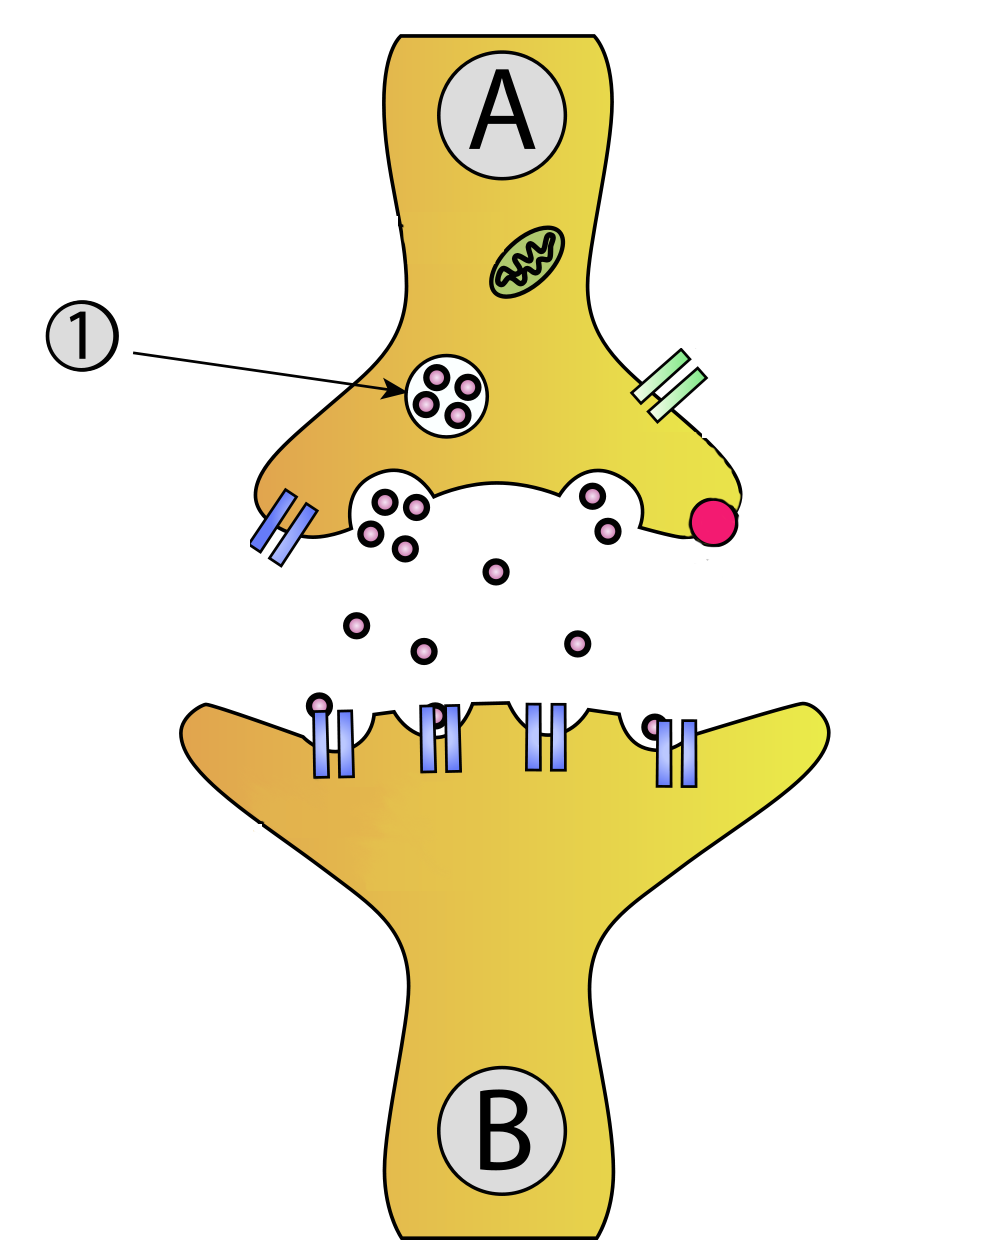
\includegraphics[scale=0.2]{files/intro/img/synTransmitter.png}
	\caption{To nerveceller, en afsender af neurotransmitters (A) og en modtager (B). Pilen peger på en synaptisk vesikel.\label{fig:intro_syntrans}\cite{neuron}}
	% Original fra : http://en.wikipedia.org/wiki/File:Synapse_diag1.svg
\end{figure} 

På Centre for Stochastic Geometry and Advanced Bioimaging (CSGA) på Aarhus Universitet, forsker Professor Jens Randel Nyengaard i mikroskopier af musehjerner. 
Forskningen går ud på at undersøge hvorvidt depression er arveligt fra mor til barn hvis moderen er deprimeret under graviditeten.
En af hypotoserne i studiet er blandt andre at man ved at observere vesiklers placering i forhold til hinanden i menneskeceller, kan sige noget om en persons sandsynlighed for at blive deprimeret. Vores problem går ud på at undersøge i hvilket omfang det kan lade sig gøre at detektere vesiklerne i cellerne.
%og lave et system der kan hjælpe forskere med at detektere disse vesikler i en celle.
Herefter vil andre efterfølgende kunne bruge denne detektion af vesikler til at analysere deres placering i forhold til hinanden, og automatisere proceduren.

Til at fremstille billederne af vesiklerne benyttes et elektronmikroskop der tager et mikroskopi af en hjerne der er frosset ned til mellem -150$^\circ$ C og -238$^\circ$ C . Disse mikroskopier er lavet ved at dele hjernen op i mange forskellige "lag" af mikroskopier.
Der vil således forekomme skygger af nerveceller fra højere eller lavere lag på et givent billede.
Da elektronmikroskopet tager billeder af mikroskopier ved meget lave temperaturer undgår man at skade cellerne unødigt, da cellerne er meget følsomme overfor stråling, der foresager meget støj i billederne. Der forekommer stadig en del støj hvilket også fremgår af billedet i figur \ref{fig:intro_celler}.
Et eksempel på en nervecelle med vesikler inden i er markeret i figuren. 
\begin{figure}[H]
	\centering
	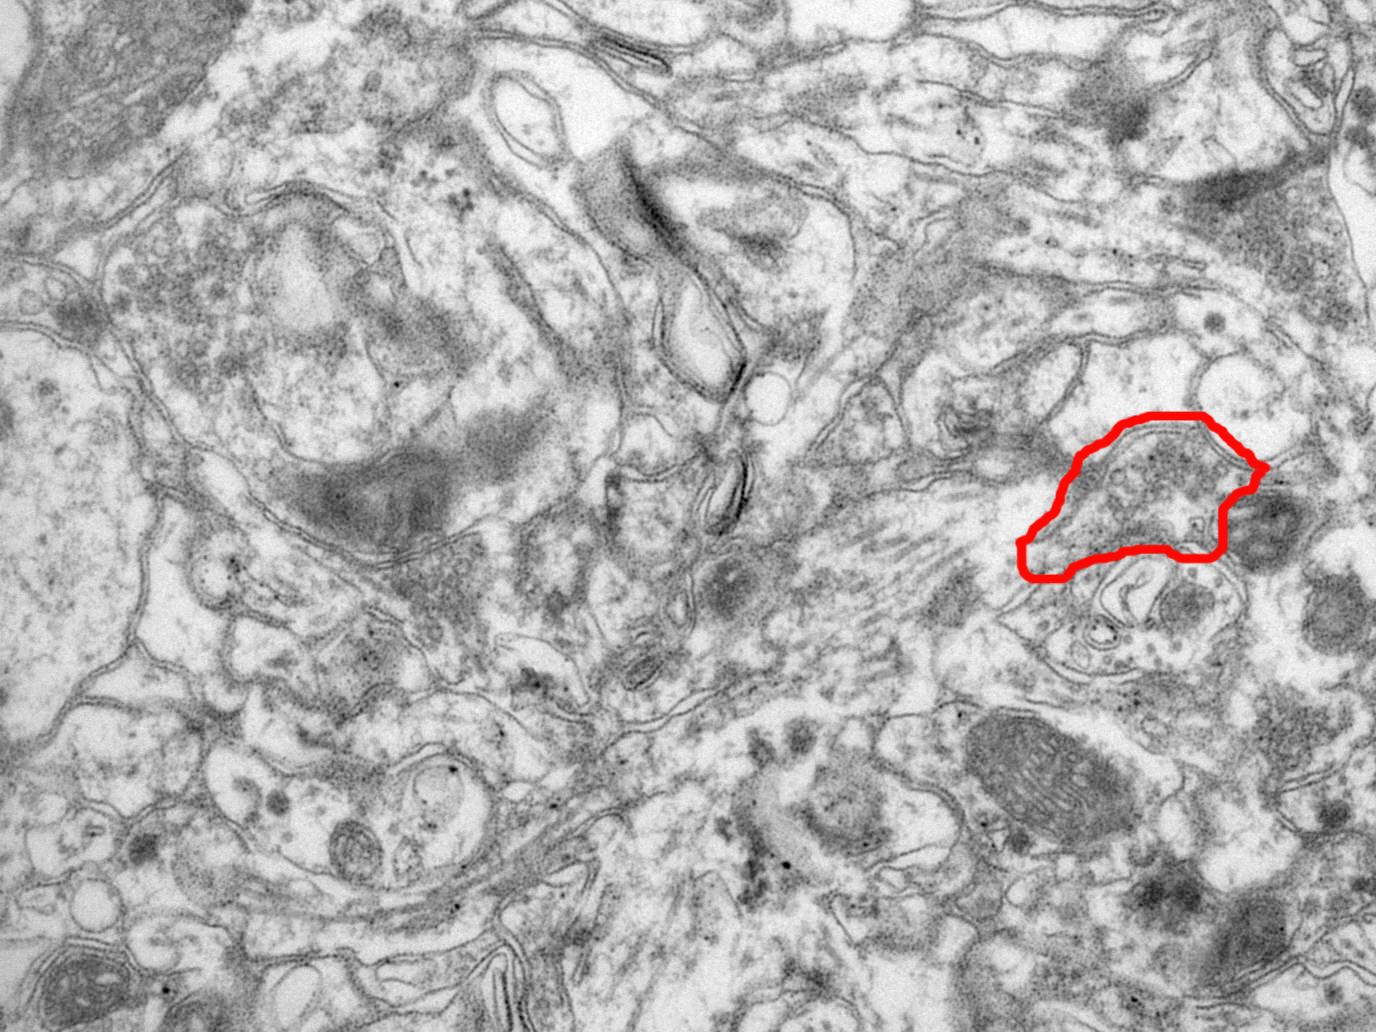
\includegraphics[scale=0.5]{files/intro/img/celler2.png}
	\caption{Billede af nerveceller taget med et elektronmikroskop. I billedet er der markeret en celle med rødt.\label{fig:intro_celler}}
\end{figure}

\subsection{Ground truth}				
Vi ønsker at detektere synaptiske vesikler i celler, og er derfor kun interesseret i billeder der indeholder en enkelt celle. Billedet til venstre i figur \ref{fig:intro_celle_groundtruth} viser et sådan udsnit. Grundet den høje støj omkring vesiklerne, er det svært at se hvor der er en vesikel, og hvor der bare er støj fra de omkringliggende vesikler eller andet som tilsammen ligner en ny vesikel. Derfor har vi i samarbejde med Professor Jens Randel Nyengaard markeret ground truth i de billeder vi behandler. Et af disse ses til højre i figur \ref{fig:intro_celle_groundtruth} hvor ground truth er markeret med lyserød prikker i hver vesikel.

\begin{figure}[H]
	\begin{minipage}[b]{0.5\linewidth}
		\centering
		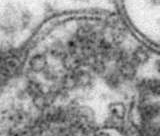
\includegraphics[scale=1.5]{files/intro/img/celle.png}
	\end{minipage}
	\hspace{0.5cm}
	\begin{minipage}[b]{0.5\linewidth}
		\centering
		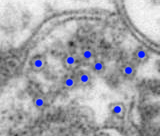
\includegraphics[scale=1.5]{files/intro/img/celle_groundtruth.png}
	\end{minipage}
	\caption{Venstre: udsnit af en enkelt nervecelle. Højre: samme udsnit med ground truth markeret med lyserøde prikker.\label{fig:intro_celle_groundtruth}}
\end{figure}

Hvis man med sine egne øjne ikke kan skelne vilkårlig støj fra en kant, vil det naturligvis også være svært at detektere alle vesikler korrekt ved hjælp af billedbehandlingsteknikker. Man kan både komme til at klassificere nogle områder der ligner en vesikel meget, men ikke er det, og omvændt kan man undlade at klassificere en vesikel, da området omkring den har så meget støj at det er svært at skælne hvor kanten stopper og støjen starter. 

\begin{figure}[H]
	\centering
	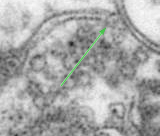
\includegraphics[scale=1.5]{files/intro/img/celle_questionves.png}
	\caption{Er der en vesikel for enden af pilen?\label{fig:intro_celle_question}}
\end{figure}

Et eksempel på et område hvor det er svært at se hvorvidt der er en vesikel ses i figur \ref{fig:intro_celle_question}. Øverst i billedet ses to områder med parallele linjer. Området mod venstre er kanten på cellen hvori vi ønsker at detektere vesikler. Den anden er kanten fra en anden celle der går lidt indover vores celle. Pilen peger så mod et område hvor de to kanter mødes, og der er meget støj. Det er svært at se med det utrænede øje hvorvidt dette er en vesikel eller bare støj. Yderligere er billederne taget ud fra meget tynde udsnit af hjernen, og det kan forekomme at man kan se skyggen af en vesikel eller celle der hører til et andet snit.  

Vores målsætning er derfor ikke at finde ground truth i alle billeder, uden at detektere en eneste falsk positiv vesikel. Succeskriteriet er blot at finde størstedelen af vesiklerne, og holde antallet af falske positiver nede.   

%% Kildehenvisninger
% http://en.wikipedia.org/w/index.php?title=Synaptic_vesicle&oldid=422206613
% http://en.wikipedia.org/w/index.php?title=Neurotransmitter&oldid=429460993
% http://en.wikipedia.org/w/index.php?title=Neuron&oldid=427379524
% http://en.wikipedia.org/w/index.php?title=Cryogenics&oldid=428358887
% http://en.wikipedia.org/w/index.php?title=Cryo-electron_microscopy&oldid=425946253


